% !TEX root = ../thesis.tex
%
\chapter{Concepts}
\label{sec:concepts}

\cleanchapterquote{Q: What's the difference between machine learning and statistics?\\A: ConvNets}{Bored Yann LeCun}{via Twitter}

\section{Machine learning}
\label{sec:concepts:ml}

\section{Neural Networks}
\label{sec:concepts:nn}

\subsection{Convolutions} % (fold)
\label{sub:conepts:nn:conv}

\subsection{Activation Functions} % (fold)
\label{sub:conepts:nn:activations}
\gls{relu}

\subsection{Regularization} % (fold)
\label{sub:conepts:nn:regularization}

\subsection{BatchNorm} % (fold)
\label{sub:conepts:nn:batchnorm}
Batch normalization \citep{ioffe_batch_2015} is a method the ease the computation of gradient decent in backpropagation. Inside a deep neural network emerges the problem of internal covariate shift. Each deeper layer of the network depends on the outputs from its previous layer. The first layer learns on top of the data input but the second layer learns from the output of the first layers features and the third layer depends on the second one and so on. In training all these features change through backpropagation and so the the distribution of all activations change and the deeper the layer the longer the chain of evolving distributions in front of it is.\\
If the features in training shift over time the gradient decent becomes harder as each layer has to follow this covariate shift of its successor. Batch norm helps to avoid this difficulty by normalizing mini batches of inputs. The layer is added after a convolutional layer (or any other linear layer) and collects a batch of inputs $B = \{x_1, x_2, x_3, \dots, x_n\}$ for this layers inputs. Then it calculates the mean $\mu_B$ and the variance $\sigma_B^2$ for this mini batch. Normalizing all the values from that batch  with
\begin{equation}
    \hat{x_i} = \frac{x_i - \mu_b}{\sqrt{\sigma_B^2 + \epsilon}}
\end{equation}
($\epsilon$ is added to avoid divisions by zero) yields the output $\{\hat{x_1},\dots,\hat{x_n}\}$.\\
To use the batch norm parameters in testing time we compute a moving average over the means and variances of the batches while testing. The forward pass uses these averages to normalize the test inputs.

\section{Fully Convolutional Networks}
\label{sec:concepts:fcn}

\subsection{Deconvolution} % (fold)
\label{sub:conepts:fcn:deconv}
Deconvolution or often called transposed convolution, first used by \citet{zeiler_deconvolutional_2010}, introduces a new operation for neural networks.

\begin{figure}[h]
    \centering
    \begin{tabular}{cc}
    \begin{tikzpicture}[font=\footnotesize\sffamily]
        \fill[black!20] (1,3) rectangle (2,3.5);
        \fill[black!20] (6,3) rectangle (7,3.5);

        \foreach \x/\y in {1/2, 2/1.5, 3/1, 4/0.5, 5/0}
            \fill[set2_1!50] (\x, \y) rectangle (\x + 2, \y + 0.5);

        \fill[black!20] (1,2) rectangle (2,2.5);
        \fill[black!20] (6,0) rectangle (7,0.5);

        \foreach \x/\y in {1/2, 2/1.5, 3/1, 4/0.5, 5/0}
        {
            \node[above right] at (\x + 0.0, \y) {1};
            \node[above right] at (\x + 0.5, \y) {2};
            \node[above right] at (\x + 1.0, \y) {3};
            \node[above right] at (\x + 1.5, \y) {4};
        }

        \draw[step=0.5cm,gray,very thin] (0,0) grid (0.5,2.5);
        \draw[step=0.5cm,gray,very thin] (0.99,2.99) grid (7,3.5);
        \draw[step=0.5cm,gray,very thin] (0.99,0) grid (7,2.5);
        \draw [->] (2.25,3.25) -- (2.25,2);
        \draw [->] (2.75,3.25) -- (2.75,2);
        \draw [->] (3.25,3.25) -- (3.25,2);
        \draw [->] (3.75,3.25) -- (3.75,2);
        \draw [->] (1.9,1.75) -- (0.5,1.75);
    \end{tikzpicture} &
    \begin{tikzpicture}[font=\footnotesize\sffamily]
        \fill[black!20] (0,5) rectangle (0.5,6);
        \fill[black!20] (0,0) rectangle (0.5,1);

        \foreach \y/\x in {4/1, 3/1.5, 2/2, 1/2.5, 0/3}
            \fill[set2_1!50] (\x, \y) rectangle (\x + 0.5, \y + 2);

        \fill[black!20] (1,5) rectangle (1.5,6);
        \fill[black!20] (3,0) rectangle (3.5,1);

        \foreach \y/\x in {4/1, 3/1.5, 2/2, 1/2.5, 0/3}
        {
            \node[above right] at (\x, \y + 1.5) {1};
            \node[above right] at (\x, \y + 1.0) {2};
            \node[above right] at (\x, \y + 0.5) {3};
            \node[above right] at (\x, \y) {4};
        }

        \draw[step=0.5cm,gray,very thin] (0.99,6.49) grid (3.5,7);
        \draw[step=0.5cm,gray,very thin] (0,0) grid (0.5,6);
        \draw[step=0.5cm,gray,very thin] (0.99,0) grid (3.5,6);
        \draw [->] (1.25,6.75) -- (1.25,5);
        \draw [->] (1.75,6.75) -- (1.75,5);
        \draw [->] (1,4.75) -- (0.5,4.75);
        \draw [->] (1,4.25) -- (0.5,4.25);
    \end{tikzpicture} \\[6pt]
    (a) Convolution & (b) Transposed Convolution
    \end{tabular}
    \caption{Convolution with stride 2 in 1D and transposed convolution with stride 2. Input signals are at the top, output is to the right and the gray boxes are padding. With the arrows we note how input points contribute to the output. The convolution applies a filter of size 4 to an signal of size 8 and with the padding produces an output of size 5. The transposed convolution in return takes a input of 5 and returns a signal of size 10. Figure is based on \citep{shi_is_2016}.}
    \label{fig:1d_strided_conv}
\end{figure}

For images the output size of a deconvolutional (deconv) layer is calculated with the inverse formula for the output size of a convolutional layer. The stride defines the upsampling factor of this layer, the kernel size the ratio of 'overlapiness' and the padding is set accordingly.

\subsection{Fully convolutional network} % (fold)
\label{sub:conepts:fcn:fcn}
Proposed by \citet{long_fully_2015} \glspl{fcn} are a specific architecture of CNNs. Fully convolutional states that the network consists only of convolutional layers. As these are translation invariant the networks can take arbitrarily sized inputs and produce a coarse output.\\
The original authors use this architecture for semantic segmentation which means to assign each pixel in an image a semantic label (dog, person, tree, etc.). They build their network from classic semantic object classifiers like VGG-16 \citep{simonyan_very_2014}. These take fixed sized images as inputs and produce a single label thereby classifying the whole image. Typically these networks produce high level features through a series of convolutional layers and classify them with a single or a series of fully connected layers (inner product of the inputs). To label an image pixel-wise with such an architecture we would have to forward the neighborhood of each pixel through the network which would introduce an \bigO{w * h} time complexity ($w$ and $h$ being the width and the height of the image).

\subsubsection{Conversion of \gls{fc} layers}
\gls{fc} layers can directly be converted into \gls{conv} layers which makes \glspl{fcn} immensely efficient. To understand this process let us examine the VGG-16 network. After the 13 \gls{conv} layers and 5 max-pooling layers we get an output from \texttt{pool5} with size $512\times7\times7$. Through pooling the original images ($224\times224$) got reduced to $7\times7$ images over 512 channels. These go though 3 \gls{fc} layers. The first \gls{fc} layer returns 4096 values. To convert this we replace it with a \gls{conv} layer with kernel size 7 and 4096 channels thus resulting also in $1\times1\times4096$ output volume. The weights from the \gls{fc} layer can be reshaped into the size of the \gls{conv} layer. The other to \gls{fc} layers with 4096 and 1000 outputs, respectively can directly be put into convolutions with kernel size 1.
For the normal $224\times224$ images nothing changed as the output of the first \gls{fc} layer is still the 4096 values but if we now increase the data size to e.g. the double $448\times448$ the advantage becomes apparent. The \texttt{pool5} will return $14\times14$ images and the new \gls{conv} layer will just slide over the bigger images returning $8\times8$ images. Lastly the other $1\times1$ convolutions do not change the size so that we get 64 predictions over the 1000 classes instead of one. These are the same as if we would have slided a window over the original image with an $8\times8$ grid but because the computations on the GPU are shared for the $7\times7$ kernels we heavily increased performance compared to the naïve solution.

\section{Residual Networks}
\label{sec:concepts:resnet}
After the succes of AlexNet \citep{krizhevsky_imagenet_2012} and with the possibilities of fast GPU computing neural networks got deeper and bigger.
The VGG-16 by \citet{simonyan_very_2014} has 442.5 million trainable parameters for its 16 layers. The more parameters a network has the harder the training becomes.
Since the last years multiple new network architectures were developed that achieve higher accuracy with less parameters and therefore shorter inference time \citep{canziani_analysis_2016}. One of those architectures are \gls{resnet} by \citet{he_deep_2016} with which they won the COCO  \citet{lin_microsoft_2014-1} and the ImageNet \citet{russakovsky_imagenet_2015} object detection challenges in 2015.
A \gls{conv} layer in a standard feed forward network learns a mapping $\mathcal{H}(x)$ from its input $x$. When training the network we reach the point at which the accuracy saturates. At this point the layers which are further trained should approximate a identity mapping of their inputs as the optimum has already been reached. In practice with deep networks new layers at some point in training rapidly mode away from the identity they should learn and degrade the training error after it already saturated. Thus making these networks deeper will worsen their results \citep{he_convolutional_2015}.
\begin{figure}
    \centering
    \begin{tabular}{p{6cm}p{6cm}}
    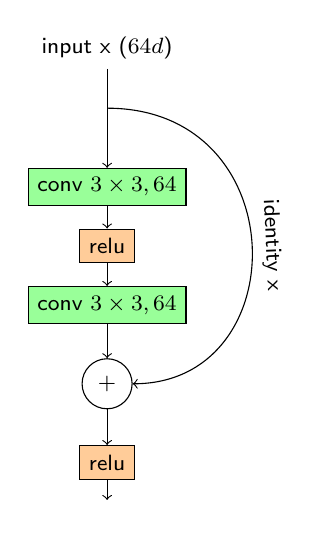
\begin{tikzpicture}[font=\footnotesize\sffamily]
        \path (0, 5) node[above](xinp) {input x ($64d$)}
              (0, 3.5) node[fill=green!40, draw](xc1) {\gls{conv} $3\times3, 64$}
              (0, 2.75) node[fill=orange!40, draw](xr1) {\gls{relu}}
              (0, 2) node[fill=green!40, draw](xc2) {\gls{conv} $3\times3, 64$}
              (0, 1) node[circle,draw](xplus) {+}
              (0, 0) node[fill=orange!40, draw](xend) {\gls{relu}}
              (0, -0.6) node(xout) {};
        \draw[->] (xinp) -- (xc1);
        \draw[->] (xc1) -- (xr1);
        \draw[->] (xr1) -- (xc2);
        \draw[->] (0, 4.5) .. controls +(right:2.4cm) and +(right:2.4cm) .. node[sloped, above] {identity x} (xplus);
        \draw[->] (xc2) -- (xplus);
        \draw[->] (xplus) -- (xend);
        \draw[->] (xend) -- (xout);
    \end{tikzpicture} &

    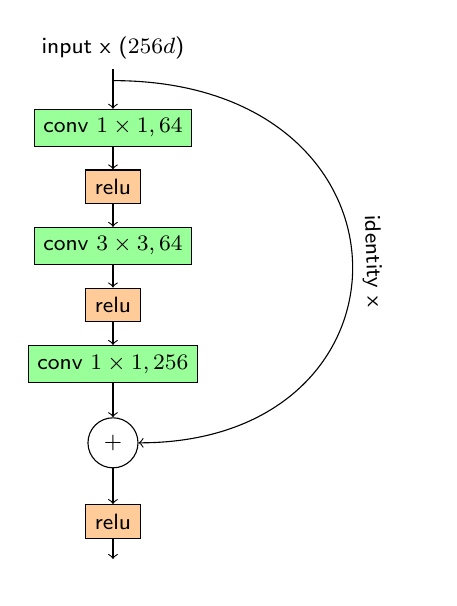
\begin{tikzpicture}[font=\footnotesize\sffamily]
        \path (0, 5.75) node[above](xinp) {input x ($256d$)}
              (0, 5) node[fill=green!40, draw](xc1) {\gls{conv} $1\times1, 64$}
              (0, 4.25) node[fill=orange!40, draw](xr1) {\gls{relu}}
              (0, 3.5) node[fill=green!40, draw](xc2) {\gls{conv} $3\times3, 64$}
              (0, 2.75) node[fill=orange!40, draw](xr2) {\gls{relu}}
              (0, 2) node[fill=green!40, draw](xc3) {\gls{conv} $1\times1, 256$}
              (0, 1) node[circle,draw](xplus) {+}
              (0, 0) node[fill=orange!40, draw](xend) {\gls{relu}}
              (0, -0.6) node(xout) {};
        \draw[->] (xinp) -- (xc1);
        \draw[->] (xc1) -- (xr1);
        \draw[->] (xr1) -- (xc2);
        \draw[->] (xc2) -- (xr2);
        \draw[->] (xr2) -- (xc3);
        \draw[->] (0, 5.6) .. controls +(right:4cm) and +(right:4cm) .. node[sloped, above] {identity x} (xplus);
        \draw[->] (xc3) -- (xplus);
        \draw[->] (xplus) -- (xend);
        \draw[->] (xend) -- (xout);
    \end{tikzpicture}
    \\[6pt]
    (a) A simple non-linear residual block. & (b) A bottleneck block as employed in the deeper \glspl{resnet}.
    \end{tabular}

    \caption{Two examples of residual blocks. The input of the block is fused into the ouptut of the last \gls{conv} layer and added element-wise channel-per-channel onto it. A \gls{relu} is trailing the sum again.}
    \label{fig:resblock}
\end{figure}


The main idea of \glspl{resnet} is pretty simple. They are build from many small identical blocks of which one example is shown in \figreft{fig:resblock}. Instead of blocks that learn the mapping $\mathcal{H}(x)$ we introduce blocks that learn the \textit{residual} $\mathcal{F}(x) = \mathcal{H}(x) - x$ of this mapping. For that we add skip connections between the input and the output of these blocks so that the input can be added to the residual that is the output of the \gls{conv} layers. Learning the residual instead of the actually mapping has the advantage that if new \gls{conv} layers are added and stay unlearned the whole residual block still yields the identity mapping which will not lead to the degradation problem we see with normal deep networks.

\subsection{Network design}
\label{sec:concepts:resnet:design}
Using the basic concept of residual blocks we build a successful architecture. First lets look at what the blocks can contain. The first example in \figreft{fig:resblock} uses just two \gls{conv} layers and a \gls{relu} to learn the residual. Therefore the block is described by:
\begin{equation}
    \mathcal{F}(x) = W_2\sigma(W_1 x + b_1) + b_2
\end{equation}
The $W_i$ and $b_i$ denote the weights and biases for the two layers, respectively and the$\sigma$ denotes the \gls{relu} layer thus making the block non-linear. Actually any chain of layers could be used to model the residual mapping. One could use this technique with just one \gls{conv} layer but as the original authors \citep{he_deep_2016} depict, this will just result in a normal linear projection which does not improve performance compared to a normal network.

Deeper networks will become in more complex. We want to limit the increase in complexity. This can be done with bottleneck blocks as the second example in \figreft{fig:resblock}. Here we use $1\times1$ \gls{conv} layers to first reduce the dimensionality of the input and to increase it again to the inputs dimension. The actual mapping convolution now has a smaller input dimension.
\newcommand{\resblock}[2]{$
    \begin{bmatrix}
        \text{1$\times$1, #2}\\[-.1em]
        \text{3$\times$3, #2}\\[-.1em]
        \text{1$\times$1, #1}
    \end{bmatrix}
$}
\begin{figure}
    \begin{tikzpicture}[font=\footnotesize, node distance=0.3cm]
        {[start chain]
           \node[on chain,draw,text width=1.5cm] (conv1) {$7\times7$, 64\newline stride 2};
           \node[on chain,draw,join=by {->},text width=2.7cm] (pool) {$3\times3$ max pool\newline  stride 2};

           \node[on chain,draw,join=by {->}] (RB1) {\resblock{256}{64}};
           \node[below=0.8cm] at (RB1) {$\times$ 3};
           \node[above=1cm,draw,minimum width=2cm] at (RB1) {$56\times56$};

           \node[on chain,draw,join=by {->}] (RB2) {\resblock{512}{128}};
           \node[below=0.8cm] at (RB2) {$\times$ 4};
           \node[above=1cm,draw,minimum width=2cm] at (RB2) {$28\times28$};

           \node[on chain,draw,join=by {->}] (RB3) {\resblock{1024}{256}};
           \node[below=0.8cm] at (RB3) {$\times$ 6};
           \node[above=1cm,draw,minimum width=2cm] at (RB3) {$14\times14$};

           \node[on chain,draw,join=by {->}] (RB4) {\resblock{2048}{512}};
           \node[below=0.8cm] at (RB4) {$\times$ 3};
           \node[above=1cm,draw,minimum width=2cm] at (RB4) {$7\times7$};
        }
    \end{tikzpicture}
    \caption{Each bottleneck block has three \gls{conv} layers with their kernel sizes and channel count denoted in the graph. Beneath each block is the recurrence written and above are the output sizes for these blocks.
 }
    \label{fig:resnet50}
\end{figure}

For this work we use the 50-layered \gls{resnet} as described in the original paper. Its architecture is shown in \figreft{fig:resnet50}.
